\chapter{Supplemental material}
\label{app:supplemental}

\section{Other measures of uncertainty in estimation theory}
\label{sec:otheruncertainty}

The fact that different measures of uncertainty inform us about different aspects of some estimation problem is well known, both in classical \citep{jaynes2003} and quantum \cite{iwo1993} scenarios. Among all the available options, in the literature of quantum metrology one typically finds a clear distinction between frequentist and Bayesian uncertainties \cite{rafal2015, li2018}, which in practice are associated, respectively, with a high amount of prior information, in which case we say that they are \emph{local}, and with a low amount of prior knowledge, meaning that they are \emph{global} \cite{paris2009, haase2018jul}. However, we can also find studies including both local and global tools without introducing the former distinction \cite{hall2012}. In addition, it is common to associate the idea of fixed but unknown parameters with the frequentist approach, while Bayesian metrology is seen as if we were giving a random description of such parameters \cite{rafal2015}. Nevertheless, Bayesian uncertainties also admit parameters that are fixed but unknown, as our discussion in section \ref{sec:uncertainty} and the work in \cite{li2018} show.   

In view of this, a more transparent picture of the different types of uncertainty and how they should be used in metrology has a great potential in terms of establishing meaningful comparisons between optimal protocols. This is precisely one of the key advantages of the three-step method to construct uncertainties that we have proposed in the main text\footnote{Nonetheless, note that our selection of uncertainties in section \ref{sec:uncertainty} has been motivated by the practical requirements of our problem, and it does not include important alternatives such as the use of entropic uncertainty relations \cite{jizba2016, jizba2017, hall2018}.}. 

Interestingly, shortly after the development of our three-step construction (which we originally published in \cite{jesus2017} in the context of the algorithm in section \ref{subsec:numalgorithm}), a related approach was proposed by Li \emph{et al.} \cite{li2018}\footnote{However, both our work \cite{jesus2017} and \cite{li2018} are based on the square error and a single parameter, while the discussion in section \ref{sec:uncertainty} is more general.}. The authors of \cite{li2018} classified the uncertainties in terms of frequentist and Bayesian quantities, and, within each group, in terms of random and fixed parameters. This allowed them to analyse the mathematical relationships between uncertainties, and to establish which bounds are satisfied by different errors. 

The errors that Li \emph{et al.} identify for Bayesian metrology with fixed parameters are equivalent to those that we have presented in section \ref{sec:uncertainty} (and in our work \cite{jesus2017}). The other groups are useful to understand the origin of the paradoxes that can emerge when bounds that are only valid for certain quantities are misapplied \cite{li2018}. Still, notwithstanding the merits of this extended classification, it can be argued that our three fundamental categories provide a simpler perspective without a practical loss of generality.

For example, let us take the case of random parameters. In these schemes the experiment is repeated $\nu$ times, such that we make $\mu$ observations per repetition, and the random component appears because the unknown parameters can have different values in each repetition \cite{li2018}. The deviation function in this situation is \cite{martinezvargas2019}
\begin{equation}
\frac{1}{\nu} \sum_{i = 1}^\nu \mathcal{D}\left[\boldsymbol{g}(\boldsymbol{m}_i), \boldsymbol{\theta}_i \right].
\end{equation}
According to our discussion, a theorist that is designing the experiment needs a probability with information about outcomes and parameters. Suppose we have the distribution of the different values that the random parameters can acquire. The parameters may change when we rerun the experiment, but they remain fixed while we are generating the measurement outcomes $\boldsymbol{m}_i$ during the $i$-th repetition \cite{li2018}. If $\boldsymbol{\theta}_i$ represents the fixed but unknown values of that trial, then we know how likely is the appearance of each of the possible values that they could have acquired in that particular iteration, and thus we can encode the information about their random distribution in the prior $p(\boldsymbol{\theta}_i)$, provided that nothing else is known. Combining this with the likelihood $p(\boldsymbol{m}_i|\boldsymbol{\theta}_i)$, and noticing that the previous argument is identical for all the iterations of the experiment, we find the error
\begin{equation}
\frac{1}{\nu} \sum_{i = 1}^\nu \int d\boldsymbol{\theta}_i d\boldsymbol{m}_i ~ p(\boldsymbol{\theta}_i, \boldsymbol{m}_i) ~\mathcal{D}\left[\boldsymbol{g}(\boldsymbol{m}_i), \boldsymbol{\theta}_i \right].
\label{randomerr}
\end{equation}
Finally, by noting that the previous expression sums the same numerical uncertainty $\nu$ times, we conclude that equation (\ref{randomerr}) is formally identical to equation (\ref{errthe}). That is, we arrive to the known result that we can model either random or fixed but unknown parameters with the same mathematics in the context of a theoretical study, even when they are physically different situations. The crucial observation is that the previous analysis is simply a combination of $\nu$ scenarios, each of them belonging to our third type of uncertainty in section \ref{sec:uncertainty}.  

The case of frequentist uncertainties is more subtle. Frequentist metrology is based on the error \cite{paris2009, rafal2015, li2018}
\begin{equation}
\int d\boldsymbol{m}~p(\boldsymbol{m}|\boldsymbol{\theta}) ~\mathcal{D}[\boldsymbol{g}(\boldsymbol{m}),\boldsymbol{\theta}].
\label{freqerror}
\end{equation}
As noted in \cite{jaynes2003}, this is the error to be employed when we do not have access to a set of specific outcomes but we do know $\boldsymbol{\theta}$, which in principle is a different type of problem. However, it can be shown \cite{hall2012, rafal2015, kolodynski2014, haase2018jul} that if certain assumptions are fulfilled in a local region of the parameter domain, often combined with an asymptotic requirement of many repeats or copies, then the quantity in equation (\ref{freqerror}) can be made useful for parameter estimation in a wide range of practical cases. Its key advantage is that the related calculations are generally more tractable than the alternatives, but, at the same time, it can be argued that it is also physically unsatisfactory. To see why, note that $p(\boldsymbol{\theta})$ does not appear in equation (\ref{freqerror}), and yet knowledge about the local region of interest is precisely the type of prior information that is best represented with a prior probability. 

Furthermore, our calculations in previous chapters strongly suggest that, for metrology protocols, the local regime emerges naturally from the Bayesian error in equation (\ref{errthe}) whenever the appropriate conditions are fulfilled, which is in agreement with other studies that also connect Bayesian and non-Bayesian quantities in quantum metrology \cite{jarzyna2015true}. From a formal perspective, this behaviour is a more general feature of estimation problems, and it is not limited to metrology \cite{gill2011}. In other words, we can recover the same local simplicity without sacrificing conceptual consistency and rigour, and thus there is no need to switch frameworks and use equation (\ref{freqerror}) even if we only want to work in that regime. These are our reasons to exclude equation (\ref{freqerror}) from the list of basic measures of uncertainty, a choice that differs from the path generally followed \cite{paris2009, rafal2015, li2018} (with exceptions such as the work in \cite{hall2012}). 

A final question is whether some of these uncertainties could be associated with the errors that are directly measured in the laboratory \cite{li2018}. Since our quantities are constructed out of probabilities, by virtue of the law of large numbers we know that a necessary condition is to have access to a very large amount of measurements, provided that the probabilities describe repetitive experiments. We saw an example of this when we revisited the use of the error propagation formula for phase estimation in a Mach-Zehnder interferometer (see section \ref{subsec:optint}). Otherwise, the previous quantities cannot be experimentally accessed, and they merely summarise information based on either our theoretical analysis (equations (\ref{errsim}) and (\ref{errthe})) or on empirical outcomes (equation (\ref{errexp})). The regime of limited data involves, by definition, scenarios with a low number of measurements; consequently, while our results could be implemented in practice, the uncertainties involved in their design are of a theoretical nature.   

In conclusion, it may be argued that the uncertainties examined in the classification of section \ref{sec:uncertainty} can be sufficient to accommodate a wide range of practical scenarios, including not only the cases with random parameters or a low amount of prior information, but also those with a high amount of prior knowledge (i.e., that work in the local regime) or that involve fixed parameters.

\section{How large the prior width can be such that the use of a quadratic error is justified?}
\label{prior_sinapprox_appendix}

A good experiment should be arranged such that the uncertainty $\bar{\epsilon}$ decreases as a function of the number of observations $\mu$. If the parameter to be estimated is periodic and we use the sine error 
\begin{equation}
\bar{\epsilon} = 4\int d\theta d\boldsymbol{m} ~p(\theta,m)~\mathrm{sin}^2\left[\frac{g(\boldsymbol{m})-\theta}{2} \right]
\label{sinerrcomplete}
\end{equation} 
(see section \ref{sec:uncertainty}), then the former statement implies that the greatest value acquired by $\bar{\epsilon}$ in equation (\ref{sinerrcomplete}) is given by 
\begin{equation}
\bar{\epsilon}({\mu=0}) = 4\int d\theta ~p(\theta)~\mathrm{sin}^2\left(\frac{g - \theta}{2} \right).
\label{prior_sinerr}
\end{equation}
Furthermore, equation \ref{prior_sinerr} is simplified as
\begin{equation}
\bar{\epsilon}({\mu=0}) = \frac{4}{W_0}\int_0^{W_0} d\theta ~\mathrm{sin}^2\left(\frac{g - \theta}{2} \right)
\label{priorsinerrsimple}
\end{equation}
after using the uniform prior in equation (\ref{prior_probability}) with $\bar{\theta} = W_0/2$, and the minimum of equation (\ref{priorsinerrsimple}) is achieved when the estimator $g$ satisfies $\mathrm{cos}(g - W_0) = \mathrm{cos}(g)$, which for one period implies that $g = W_0 /2$. Hence,  
\begin{eqnarray}
\bar{\epsilon}(\mu=0) = \frac{4}{W_0}\int_0^{W_0} d\theta~ \mathrm{sin}^2\left(\frac{W_0}{4} - \frac{\theta}{2} \right)
= 2\left[1 - \frac{2}{W_0}\mathrm{sin}\left( \frac{W_0}{2}\right) \right].
\label{sin_muzero}
\end{eqnarray}
If we now expand equation (\ref{sin_muzero}) up to second order in $W_0$, we find that
\begin{equation}
\bar{\epsilon}(\mu=0) \approx \frac{{W_0}^2}{12},
\label{mse_muzero}
\end{equation}  
which is the prior that we would have found using the square error directly. 

According to figure \ref{circular_mse}.i, which compares equations (\ref{sin_muzero}) and (\ref{mse_muzero}) as a function of the width $W_0$, the approximation starts to fail in a notable way when $W_0 \approx \pi$. Given that in chapter \ref{chap:nonasymptotic} we calculated the mean square error for NOON, twin squeezed vacuum and squeezed entangled states with $W_0=\pi/2$, and that $W_0=\pi/3$ was employed with both the previous states and for a coherent beam, we can say that the approximation is reasonable for these configurations when $\mu = 0$. Moreover, $\abs{g(\boldsymbol{m}) - \theta}$ will not be greater than $W_0$ for $\mu > 0$, and thus a similar reasoning could be applied to the comparison of equations (\ref{sinerrcomplete}) and (\ref{errwork}). The only scheme for which this approximation is cruder is the coherent state with prior width $W_0 = \pi$. 

\begin{figure}[t]
\centering
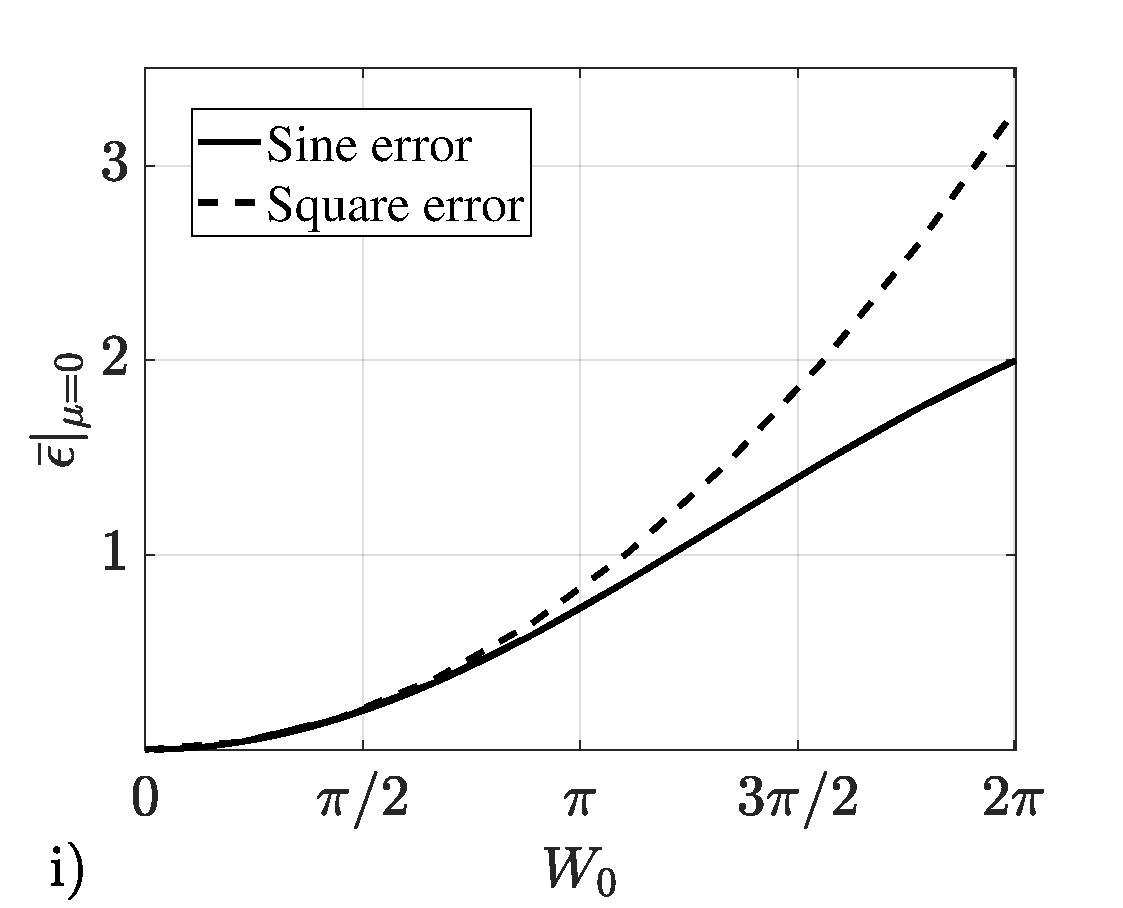
\includegraphics[trim={0.1cm 0.1cm 1.4cm 0.2cm},clip,width=7.45cm]{pictures/app_fig1i}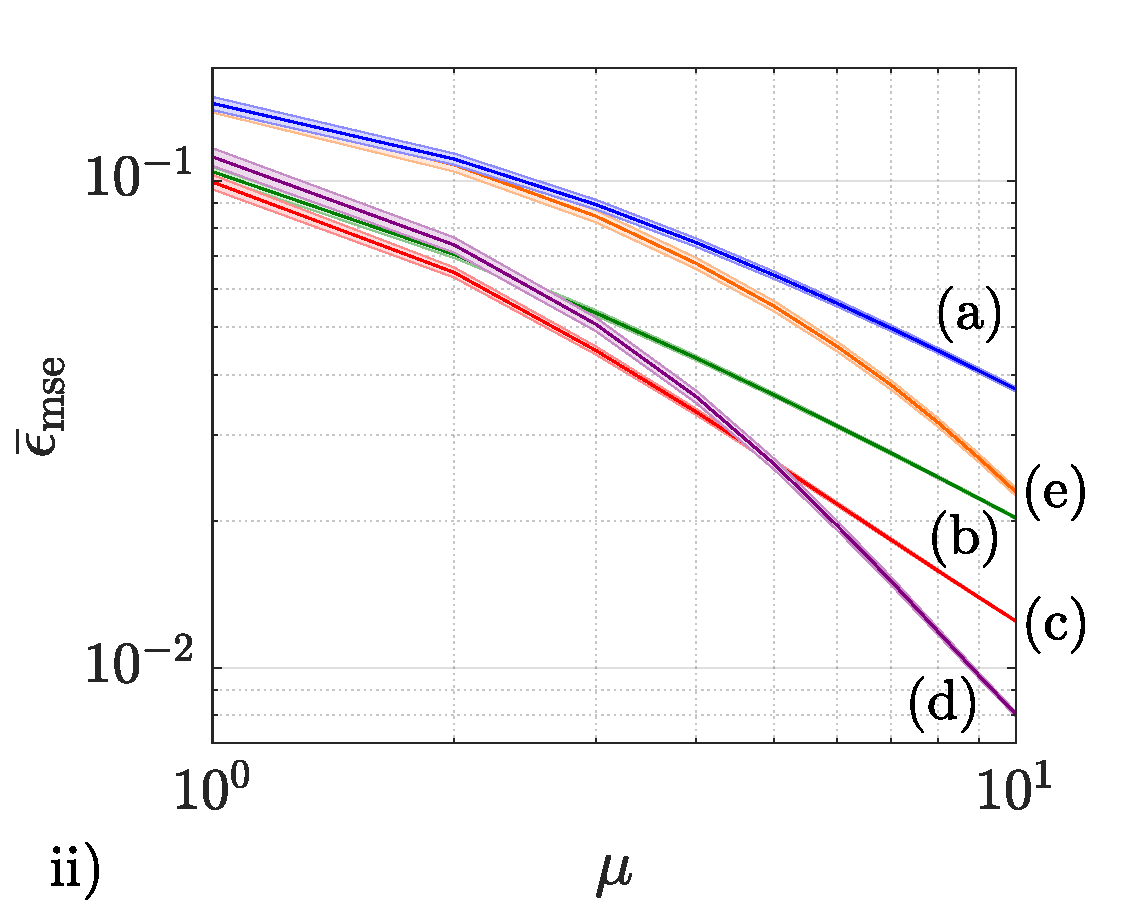
\includegraphics[trim={0.1cm 0.1cm 0.65cm 0.2cm},clip,width=7.75cm]{app_fig1ii}
	\caption[Square error as an approximation for a periodic uncertainty]{i) Comparison between the prior uncertainty ($\mu = 0$) given by a periodic error function and that associated to the mean square error as a function of $W_0$. Most of our results in Section \ref{results} are calculated using the values $W_0 = \pi/2$ and $W_0 = \pi/3$; (ii) Mean square error based on the optimal single-shot strategy (solid line) and bounds for the approximation error after having expanded the sine error up to second order (shaded area) for (a) the coherent state, (b) the NOON state, (c) the twin squeezed vacuum state, (d) the squeezed entangled state, and (e) the twin squeezed cat state, with $\bar{n} = 2$, $\bar{\theta}=0$ and $W_0 = \pi/2$. This figure shows that the mean square error is a suitable approximation for the mean sine error when we are in the regime of moderate prior knowledge.}
\label{circular_mse}
\end{figure}

A more powerful argument to refine such threshold is also possible. First we observe that the approximation $4\hspace{0.15em}\mathrm{sin}^2\lbrace\left[g(\boldsymbol{m})-\theta\right]/2 \rbrace \approx [g(\boldsymbol{m})-\theta]^2$ relies on the quantity $|g(\boldsymbol{m})-\theta|/2$ being small, where, as we have seen, $|g(\boldsymbol{m})-\theta|/2 \leqslant W_0/2$. The minimum requirement that is natural to impose is that the variable for which the Taylor expansion is calculated (i.e., $|g(\boldsymbol{m})-\theta|/2$) is slightly smaller than $1$ at most, which is always the case if the width of our experiment satisfies that $W_0 \lesssim 2$. In principle this would still be a crude approximation if we were interested in the sine function itself. However, the sine error is then integrated over all the possible values for $\theta$ and $\boldsymbol{m} = (m_1, \dots , m_\mu)$. This implies that $|g(\boldsymbol{m})-\theta|/2 \sim 2$ when $W_0\sim2$ only for a few combinations of values, and the weight of those cases will decrease as the joint probability $p(\theta,\boldsymbol{m})$ accumulates more data. We conclude then that $W_0 \lesssim 2$ is a reasonable estimation for the range of validity of the mean square error in a problem with a periodic parameter. Note that this condition has the same order of magnitude than the estimation found in \cite{friis2017}, where the authors argued that the width of their Gaussian prior had to be $\pi/2$ or less, and it is a better estimation than the one obtained in the previous paragraphs. 

From the previous discussion we see that only the calculation of the first few shots could be potentially misleading if we use the mean square error. To show that this is not the case for the type of schemes analysed in the main text, let us estimate explicitly the error of the Taylor expansion for some of the schemes in chapter \ref{chap:limited}. First, using Taylor's theorem we have that $\mathrm{sin}^2(x) = x^2-x^4 \mathrm{cos}(2\varepsilon)/3$, where $\varepsilon \in [0,x]$  \cite{mathematics2004}. The first term is the approximation that we want to use, while the second term represents the error of this approximation. Using the fact that the cosine is bounded between $-1$ and $1$, the Taylor error can be estimated with 
\begin{equation}
\Delta \bar{\epsilon} = \frac{1}{12}\int d\theta d\boldsymbol{m}~p(\theta) p(\boldsymbol{m}|\theta) \left[g(\boldsymbol{m})-\theta\right]^4,
\label{taylorerror}
\end{equation}
and knowing that the optimal phase estimator is the average of the posterior probability $p(\theta|\boldsymbol{m}) \propto p(\theta)p(\boldsymbol{m}|\theta)$, we can rewrite equation (\ref{taylorerror}) as
\begin{equation}
\Delta \bar{\epsilon} = \frac{1}{12}\int d\theta' p(\theta') \int d\boldsymbol{m}~ p(\boldsymbol{m}|\theta') \Delta \bar{\epsilon}(\boldsymbol{m}),
\end{equation}
where
\begin{equation}
\Delta \bar{\epsilon}(\boldsymbol{m}) = \langle \theta^4 \rangle- 4 \langle \theta \rangle \langle \theta^3 \rangle + 6\langle \theta \rangle^2 \langle \theta^2 \rangle - 3\langle \theta \rangle^4
\end{equation}
and we have used the notation $\left\langle \Box \right\rangle = \int d\theta p(\theta|\boldsymbol{m}) \Box$. This is precisely the three-step decomposition introduced in section \ref{subsec:numalgorithm} to obtain the mean square error and, as such, we can compute $\Delta \bar{\epsilon}$ numerically in the same way.

This calculation is shown in figure \ref{circular_mse}.ii, where the graph in the middle of the shaded areas is $\bar{\epsilon}_{\mathrm{mse}}$ for $1\leqslant\mu \leqslant 10$ and $W_0 = \pi/2$ and the boundaries are given by $\pm \Delta \bar{\epsilon}$. We can see that the Taylor error bounds for the twin squeezed cat state, the squeezed entangled state and the twin squeezed cat state, which constitute the basis of our main results in chapter \ref{chap:limited}, do not overlap for any value of $\mu$. Therefore, all the comparisons made between these probes are valid. That the twin squeezed cat state and the coherent state overlap for $\mu = 1, 2, 3$ is not surprising, since their respective mean square errors also do (see figure \ref{bounds_results}.i), and the same observation hold for the NOON state and the squeezed entangled state when $\mu = 2$. On the other hand, the shaded area of the NOON state overlaps slightly with the top shaded area of the twin squeezed vacuum state when $\mu=1$. It is important to appreciate that the shaded areas are bounds for the Taylor error, and it is not guaranteed that the uncertainties for these two states actually coincide. However, even if they did, it would simply constitute another instance where the role of inter-mode and intra-mode correlations is altered in the regime of limited data, since a state with path entanglement that is beaten by a state with a large amount of intra-mode correlations in the asymptotic regime would reach the same uncertainty than the latter for a single shot. 

Finally, we also notice that the approximation will become even better as $W_0$ decreases, which is the case for the other prior widths that we have explored. Hence, we can conclude that the results that arise from the use of the mean square error as an approximation for the mean sine error in the regime of moderate prior knowledge are generally valid.

\section{Calculation details of some results in optical interferometry}
\label{sec:optrans}

This appendix presents the derivation of some auxiliary results employed in chapters \ref{chap:nonasymptotic} and \ref{chap:limited} for the non-asymptotic study of the Mach-Zehnder interferometer.

First we will verify that $U_{\mathrm{BS}} D_1(\alpha)\ket{0, 0} = |\alpha/\sqrt{2},-i\alpha/\sqrt{2}\rangle$. Using \cite{barnett2002}
\begin{equation}
\mathrm{exp}\left(X\right)f\left(Y\right)\mathrm{exp}\left(-X\right) = f\left[\mathrm{exp}\left(X\right)Y \mathrm{exp}\left(- X\right)\right],
\label{coherent1step}
\end{equation}
where $X$ and $Y$ are operators, we have that
\begin{align}
U_{\mathrm{BS}} D_1(\alpha) U_{\mathrm{BS}}^\dagger &= \mathrm{exp}\left(-i\frac{\pi}{2}J_x\right) \mathrm{exp}\left(\alpha a_1^{\dagger} - \alpha^{*}a_1\right) \mathrm{exp}\left(i\frac{\pi}{2}J_x\right) 
\nonumber \\
&= \mathrm{exp}\left[\alpha \left(\mathrm{e}^{-i\frac{\pi}{2}J_x}a_1^{\dagger}\mathrm{e}^{i\frac{\pi}{2}J_x}\right) - \alpha^{*}\left(\mathrm{e}^{-i\frac{\pi}{2}J_x} a_1 \mathrm{e}^{i\frac{\pi}{2}J_x}\right)\right].
\end{align}
In addition, 
\begin{align}
U_{\mathrm{BS}} a_1 U_{\mathrm{BS}}^\dagger &= a_1 + \left( -i \pi/2 \right) \comm*{J_x}{a_1} + \frac{\left( -i \pi/2 \right)^2}{2!} \comm*{J_x}{\comm*{J_x}{a_1}} + \ldots = 
\nonumber \\ 
&= a_1 + i \left(\pi/4 \right) a_2 - \frac{\left(\pi/4 \right)^2}{2!} a_1 + \ldots
\nonumber \\
&= \left[ 1 - \frac{\left(\pi/4 \right)^2}{2!} + \ldots \right] a_1 + i \left[\left(\pi/4 \right) + \ldots \right] a_2
\nonumber \\
&= \mathrm{cos}\left(\pi/4\right) a_1 + i\hspace{0.1em}\mathrm{sin}\left(\pi/4\right) a_2 = \left(a_1 + i a_2\right)/\sqrt{2}
\label{opid1}
\end{align}
after combining the Baker-Campbell-Hausdorff formula \cite{yurke1986}
\begin{equation}
\mathrm{e}^{z X}Y\mathrm{e}^{-z X} =  B + z \comm*{X}{Y} + \frac{z^2}{2!} \comm*{X}{\comm*{X}{Y}} + \ldots,
\label{BCH}
\end{equation}
with the commutation relations $\comm*{a_i}{a_j} = \comm*{a_i^\dagger}{a_j^\dagger}=0$, $\comm*{a_i}{a_j^\dagger}=\delta_{ij}$ (see section \ref{subsec:qapp}). Finally, by noticing that 
\begin{equation}
\mathrm{exp}\left(-i\frac{\pi}{2}J_x\right)\ket{0, 0} = \sum_{k=0}^\infty \frac{\left(-i\pi/4\right)^k}{k!} \left( a_1^\dagger a_2 + a_1 a_2^\dagger \right)^k \ket{0, 0} = \ket{0, 0},
\end{equation}
and taking into account equations (\ref{coherent1step}) and (\ref{opid1}), we arrive at
\begin{align}
U_{\mathrm{BS}} D_1(\alpha)\ket{0, 0} &= \left[U_{\mathrm{BS}} D_1(\alpha) U_{\mathrm{BS}}^\dagger\right] U_{\mathrm{BS}}\ket{0, 0}
\nonumber \\
&= \mathrm{exp}\left\lbrace\left(\frac{\alpha}{\sqrt{2}} a_1^\dagger - \frac{\alpha^{*}}{\sqrt{2}}a_1\right) + \left[\frac{\left(-i\alpha\right)}{\sqrt{2}} a_2^\dagger - \frac{\left(-i\alpha\right)^{*}}{\sqrt{2}}a_2 \right]  \right\rbrace \ket{0, 0}
\nonumber \\
&= D_1\left(\alpha/\sqrt{2}\right)D_2\left(-i\alpha/\sqrt{2}\right) \ket{0, 0}
\nonumber \\
&= |\alpha/\sqrt{2},-i\alpha/\sqrt{2}\rangle,
\end{align}
as we expected.

On the other hand, we need to find the likelihood function $p(n_1, n_2| \theta) = ||a(n_1, n_2| \theta)||^2$ associated with the probability amplitude
\begin{equation}
a(n_1, n_2| \theta) = \langle n_1, n_2| \mathrm{e}^{-i\frac{\pi}{2}J_x}\mathrm{e}^{i N_2 \phi}\mathrm{e}^{-iJ_z\theta}\ket{\psi_{\mathrm{NOON}}} = \langle n_1, n_2| \Phi(\theta) \rangle,
\end{equation}
where $| \Phi(\theta) \rangle =  \mathrm{e}^{-i\frac{\pi}{2}J_x}\mathrm{e}^{i N_2 \phi}\mathrm{e}^{-iJ_z\theta}\ket{\psi_{\mathrm{NOON}}}$, $\phi$ is a known phase shift and $\ket{\psi_{\mathrm{NOON}}} = (\ket{N, 0} + \ket{0, N})/\sqrt{2}$. The transformation associated with the phase shifts is
\begin{equation}
\mathrm{e}^{i N_2 \phi}\mathrm{e}^{-iJ_z\theta}\ket{\psi_{\mathrm{NOON}}} = \frac{1}{\sqrt{2}}\left[\mathrm{e}^{-iN\theta/2}\ket{N, 0} + \mathrm{e}^{iN\left(2\phi + \theta\right)/2}\ket{0, N}\right],
\label{phasenoon}
\end{equation}
since
\begin{equation}
\mathrm{e}^{i N_i x}\ket{n_i} = \sum_{k=0}^\infty \frac{\left(i x\right)^k}{k!} N_i^k \ket{n_i} = \sum_{k=0}^\infty \frac{\left(i x n_i\right)^k}{k!}\ket{n_i} = \mathrm{e}^{i n_i x}\ket{n_i}.
\end{equation}
Furthermore, from
\begin{align}
U_{\mathrm{BS}} a_2 U_{\mathrm{BS}}^\dagger &= a_2 + \left( -i \pi/2 \right) \comm*{J_x}{a_2} + \frac{\left( -i \pi/2 \right)^2}{2!} \comm*{J_x}{\comm*{J_x}{a_2}} + \ldots = 
\nonumber \\ 
&= a_2 + i \left(\pi/4 \right) a_1 - \frac{\left(\pi/4 \right)^2}{2!} a_2 + \ldots
\nonumber \\
&= i\left[\left(\pi/4 \right) + \ldots \right]a_1 + \left[ 1 - \frac{\left(\pi/4 \right)^2}{2!} + \ldots \right]a_2
\nonumber \\
&= i\hspace{0.1em}\mathrm{sin}\left(\pi/4\right)a_1 + \mathrm{cos}\left(\pi/4\right)a_2 = \left(i a_1 + a_2\right)/\sqrt{2} 
\label{opid2}
\end{align}
and equations (\ref{opid1}) and (\ref{phasenoon}) we find that 
\begin{align}
| \Phi(\theta) \rangle &=  \frac{1}{\sqrt{2 N!}}\left[\mathrm{e}^{-iN\theta/2}\left(\mathrm{e}^{-i\frac{\pi}{2}J_x} a_1^\dagger \mathrm{e}^{i\frac{\pi}{2}J_x}\right)^N + \frac{\mathrm{e}^{iN\left(2\phi + \theta\right)/2}}{\sqrt{2 N!}} \left(\mathrm{e}^{-i\frac{\pi}{2}J_x} a_2^\dagger \mathrm{e}^{i\frac{\pi}{2}J_x}\right)^N \right]\ket{0, 0}
\nonumber \\
&= \frac{1}{\sqrt{2^{N+1} N!}}\left[\mathrm{e}^{-iN\theta/2}\left(a_1^\dagger - i a_2^\dagger\right)^N + \mathrm{e}^{iN\left(2\phi + \theta\right)/2}\left(-i a_1^\dagger + a_2^\dagger\right)^N \right] \ket{0, 0}
\nonumber \\
&= \frac{1}{\sqrt{2^{N+1}}}\sum_{k=0}^N \sqrt{\frac{N!}{k! (N-k)!}}\left[ \left(-i\right)^{N-k}\mathrm{e}^{-iN\theta/2} + \left(-i\right)^k \mathrm{e}^{iN\left(2\phi + \theta\right)/2} \right] \ket{k, N-k}
\nonumber \\
&= \sqrt{\frac{2}{2^N}}\sum_{k=0}^N \sqrt{\frac{N!}{k! (N-k)!}} \hspace{0.1em}\mathrm{cos}\left[N\left(\theta+\phi\right)/2 + \left(2k - N\right)\pi/4 \right] \ket{k, N \hspace{-0.1em} - \hspace{-0.1em} k}\hspace{-0.1em}.\hspace{-0.5em}
\end{align}
Hence, 
\begin{equation}
a(n, N - n | \theta) = \sqrt{\frac{2N!}{2^N n! (N-n)!}} \hspace{0.1em}\mathrm{cos}\left[N\left(\theta+\phi\right)/2 + \left(2k - N\right)\pi/4 \right],
\label{noonamplitude}
\end{equation}
where we have used that NOON states have a definite number of photons. 

If $\phi = 0$, then equation (\ref{noonamplitude}) generates the probability density
\begin{equation}
p(n,N-n|\theta) = \frac{2 N! \hspace{0.2em} \mathrm{cos}^2\left[N\theta/2 + (2n-N)\pi/4\right]}{2^N n! (N-n)!} 
\end{equation}
that we employed in chapter \ref{chap:nonasymptotic}, while for $\phi = -\pi/4$ and $N = 2$ we have that
\begin{equation}
p(n,2-n|\theta) = \frac{\mathrm{cos}^2\left[\theta + (2n-3)\pi/4\right]}{ n! (2-n)!},
\end{equation}
which is the result examined in chapter \ref{chap:limited}.

\section{Multivariate Gaussian integrals}
\label{sec:multigaussian}

Here we summarise the standard calculation of the multivariate integrals in chapter \ref{chap:networks}, which also include those in chapter \ref{chap:nonasymptotic} when we take $d=1$. 

Let us denote the classical Fisher information matrix, which it is assumed to be positive definite, by $F(\boldsymbol{\theta}')\equiv F'$, and its eigendecomposition by $F' = Z F'_D Z^\transpose$, with $F'_D=\mathrm{diag}(z_1, \dots, z_d)$. In addition, define the transformation $\boldsymbol{\theta}-\boldsymbol{\theta}' = Z \boldsymbol{y}$ between $\boldsymbol{\theta}$ and $\boldsymbol{y}$, with Jacobian $\mathrm{det}(Z) = 1$. The first calculation is
\begin{align}
G_0 &= \int_{-\boldsymbol{\infty}}^{\boldsymbol{\infty}} d\boldsymbol{\theta}\hspace{0.15em}\mathrm{e} ^{-\frac{\mu}{2}\left(\boldsymbol{\theta}-\boldsymbol{\theta}'\right)^\transpose F' \left(\boldsymbol{\theta}-\boldsymbol{\theta}'\right)} 
= \int_{-\boldsymbol{\infty}}^{\boldsymbol{\infty}} d\boldsymbol{y}\hspace{0.15em}\mathrm{e} ^{-\frac{\mu}{2}\boldsymbol{y}^\transpose F'_D \boldsymbol{y}} 
\nonumber \\
&= \prod_{i=1}^d \int_{-\infty}^{\infty} dy_i\hspace{0.15em} \mathrm{e}^{-\frac{\mu}{2}y_i^2 z_i} = \left(\frac{2\pi}{\mu}\right)^{\frac{d}{2}}  \prod_{i=1}^d \frac{1}{\sqrt{z_i}} = \left[\frac{\left(2\pi\right)^d}{\mathrm{det}(\mu F')}\right]^{\frac{1}{2}},
\label{gaussian0}
\end{align}
since $\int_{-\infty}^{\infty} dy_i\hspace{0.15em} \mathrm{e}^{-\frac{\mu}{2}y_i^2 z_i} = [2\pi/(\mu z_i)]^{1/2}$. On the other hand, 
\begin{align}
G_{1,i} &= \int_{-\boldsymbol{\infty}}^{\boldsymbol{\infty}} d\boldsymbol{\theta}\hspace{0.15em}\mathrm{e} ^{-\frac{\mu}{2}\left(\boldsymbol{\theta}-\boldsymbol{\theta}'\right)^\transpose F' \left(\boldsymbol{\theta}-\boldsymbol{\theta}'\right)}\theta_i 
= \int_{-\boldsymbol{\infty}}^{\boldsymbol{\infty}} d\boldsymbol{y}\hspace{0.15em}\mathrm{e} ^{-\frac{\mu}{2}\boldsymbol{y}^\transpose F'_D \boldsymbol{y}}  \left(\theta_i' + \sum_{j=1}^d Z_{ij}y_j\right)
\nonumber \\
&=  G_0\hspace{0.15em}\theta'_i + \sum_{j=1}^d Z_{ji}\prod_{k=1}^d \int_{-\infty}^{\infty} dy_k\hspace{0.15em} \mathrm{e}^{-\frac{\mu}{2}y_k^2 z_k}y_j =  G_0\hspace{0.15em}\theta'_i
\label{gaussian1}
\end{align}
where we have used that $\int_{-\infty}^{\infty} dy_i\hspace{0.15em} \mathrm{e}^{-\frac{\mu}{2}y_i^2 z_i}y_i = 0$. Finally, 
\begin{align}
G_{2,ij} = &~ \int_{-\boldsymbol{\infty}}^{\boldsymbol{\infty}} d\boldsymbol{\theta}\hspace{0.15em}\mathrm{e} ^{-\frac{\mu}{2}\left(\boldsymbol{\theta}-\boldsymbol{\theta}'\right)^\transpose F' \left(\boldsymbol{\theta}-\boldsymbol{\theta}'\right)}\theta_i \theta_j
\nonumber \\
= &~ \int_{-\boldsymbol{\infty}}^{\boldsymbol{\infty}} d\boldsymbol{y}\hspace{0.15em}\mathrm{e} ^{-\frac{\mu}{2}\boldsymbol{y}^\transpose F'_D \boldsymbol{y}}  \left(\theta_i' + \sum_{k=1}^d Z_{ik}y_k\right)\left(\theta_j' + \sum_{l=1}^d Z_{jl}y_l\right)
\nonumber \\
= &~ G_0\hspace{0.15em}\theta_i' \theta_j'
+ \sum_{k=1}^d \left(\theta_i' Z_{jk} + \theta_j' Z_{ik} \right)\prod_{m=1}^d \int_{-\infty}^{\infty} dy_m\hspace{0.15em} \mathrm{e}^{-\frac{\mu}{2}y_m^2 z_m}y_k
\nonumber \\
&+ \sum_{k, l=1}^d Z_{ik} Z_{jl}\prod_{m=1}^d \int_{-\infty}^{\infty} dy_m\hspace{0.15em} \mathrm{e}^{-\frac{\mu}{2}y_m^2 z_m}y_k y_l
\nonumber \\
= &~ G_0\hspace{0.15em}\theta_i' \theta_j' + \left(\frac{2\pi}{\mu}\right)^{\frac{d}{2}}  \frac{1}{\mu} \sum_{l=1}^d \frac{Z_{il} Z_{jl}}{z_l} \frac{1}{\sqrt{z_l}} \prod_{\lbrace k=1,  \hspace{0.1em} k\neq l \rbrace}^d \frac{1}{\sqrt{z_k}}
\nonumber\\
= &~ G_0 \left\lbrace\theta_i' \theta_j' + \frac{\left[\left(F'\right)^{-1}\right]_{ij}}{\mu} \right\rbrace,
\label{gaussian2}
\end{align}
given that $\int_{-\infty}^{\infty} dy_i\hspace{0.15em} \mathrm{e}^{-\frac{\mu}{2}y_i^2 z_i}y_i^2 = [2\pi/(\mu z_i)^3]^{1/2}$.

Equations (\ref{gaussian0} - \ref{gaussian2}) lead us to the results in equations (\ref{norm_asy}), (\ref{gaussiansingle}), (\ref{multigaussian0}) and (\ref{multigaussian12}) in the main text. 